\chapter{Einleitung}
\label{chap:einleitung}

\section{Grundlagen}
\label{sec:Grundlagen}
Grundsätzlich ist das in dieser Arbeit behandelnde Thema für jede Person mit einer allgemeinen Informatikausbildung ohne weiteres zu verstehen. Es wird bei dieser Personengruppe, die Kenntnisse über grundsätzliche Architekturen innerhalb der IT vorausgesetzt. Zudem kann vorausgesetzt werden, dass jede Person dieser Gruppe, der englischen Sprache mächtig ist. Trotzdem wird im weiteren Verlauf einige Begriffe genauer erklärt.
\\\\
\textbf{Time-to-Market (TTM)}\\
Unter dem Begriff Time-to-Market wird die Zeit von der Produktentwicklung bis zur Auslieferung auf dem Markt verstanden.\footnote{Vergleich mit \cite{ttm:BusinessDictionary}}  In dieser Zeit müssen Kosten für die Erstellung/Entwicklung aufgebracht werden, es wird in dieser Zeit jedoch keine Umsätze erzeugt. Daher strebt jedes Unternehmen eine möglichst geringe Time-to-Market Zeit an. Insbesondere wenn es um Wettbewerb geht, muss diese Zeit kurz gehalten werden.
\\\\    
\textbf{SOA}\\
Architekturmodell aus dem Bereich der Informatik und verteilten Systemen. Mehr dazu im Kapitel \secref{chap:soa}.
\\\\
\textbf{Microservice}\\
Wie SOA ein Architekturmodell der Informatik, welches auf verteilten Systemen aufbaut. Mehr dazu im Kapitel \secref{chap:Microservices}.
\\\\    
\textbf{Dienst (Service)}\\
Unter einem Dienst (Service) versteht man eine eigenständige Anwendung, welche seine Dienste über Schnittstellen bereitstellt.

\section{Begriffsabgrenzung}
\label{sec:Begriffsabgrenzung}

\subsection*{SOA}
Sowohl SOA als auch Microservices zählen zu den "`Service-orientierten Architekturen"'.

Die Abkürzung SOA wird hier sowohl für die Architektur allgemein, wie auch der speziellen Ausprägung verwendet.

Um die beiden Thematiken in dieser Arbeit abzugrenzen wird "`SOA"' nur als Modell verwendet und die ausgeschriebene Variante zur Kennzeichnung der Allgemeinen Architektur.

\subsection*{Microservice}
Der Begriff Microservice wird einerseits zum Beschreiben eines Architekturmodells genutzt, als auch zum beschreiben von eigenständigen Diensten (Services).

Damit keine Verwechslung entsteht, wird in dieser Arbeit der Begriff "`Microservice"' verwendet, sofern das Architekturmodell gemeint ist und der Begriff "`Dienst"' oder "`Service"', wenn ein eigenständiger Dienst gemeint ist.

\section{Motivation}
\label{sec:motivation}
Die Anforderungen an Software werden zunehmend komplexer. Sie muss nicht nur funktionieren, sondern müssen zum Teil in kürzester Zeit erweitert oder geändert werden, was eine besondere Herausforderung dar stellt. Je komplexer Software wird, desto schwieriger ist sie zu warten und zu pflegen. 

\begin{quotation}
\frqq Die Zeitspanne des Time-to-Market [(TTM)] kann [dabei] ein sehr bedeutsamer Faktor für den Erfolg des Unternehmens darstellen und ist daher nicht zu vernachlässigen. Kurze Entwicklungszeiträume bei der Time-to-Market garantieren dem Unternehmen nämlich einen Vorteil gegenüber der Konkurrenz. Hier geht es darum, dem Kunden so schnell wie möglich ein neues und innovatives Produkt anbieten zu können.
    
Um den Erfolg durch eine kurze Time-to-Market zu unterstützen und zu fördern, investieren Unternehmen in ihre Entwicklungsabteilungen. Diese können sich so nur auf ihre jeweiligen Bereiche konzentrieren. Durch eine leistungsfähige Entwicklungsabteilung kann so, in Kombination mit einem gut organisierten Projektplan und eindeutigen Zuständigkeiten, die Zeitspanne Time-to-Market so klein wie möglich gehalten werden. Gerade in Branchen, in denen Innovation eine übergeordnete Rolle spielt und der Produkt-Lebens-Zyklus generell eher kurz ausfällt, spielt eine kurze Time-to-Market eine außerordentlich wichtige Rolle.\flqq \cite{ttm}
\end{quotation}

Zusätzlich entstehen Kosten für die Planung und Entwicklung des Produktes. Bis zur Veröffentlichung des Produktes hat das Unternehmen Geld und Zeit investiert. Je länger die Zeitspanne des TTM ist, umso erfolgreicher muss das Produkt sein, bzw. der Preis groß genug sein, damit möglichst zeitnah der Break-even-Point, also die Schwelle, ab der die Produktionskosten wieder eingenommen worden sind und ein Gewinn entsteht, erreicht wird.

Zudem gibt es in einem Unternehmen nicht nur ein Software Produkt, sondern eine viel Zahl verschiedener Produkte für unterschiedliche Anwendungsfälle. Dabei kann es passieren, dass einige Anwendungen gleiche Funktionalitäten beinhalten. Müssen solche Funktionalitäten geändert werden, müssen dafür alle Anwendungen, welche diese Funktionen bereitstellen, geändert werden. Einfacher ist es daher, nur eine Anwendung zu haben, welches diese Funktionalität anbietet. Dadurch bedarf es nicht mehr die Anpassung von vielen Anwendungen, sondern nur noch von dieser einen.

\section{Ausgangssituation}
\label{sec:ausgangssituation}
Bei der Ausgangssituation gehen wir von einem fiktiven Szenario aus, welche an das aus \cite[S. 15]{EWolff2016:Microservices} angelehnt ist und im wesentlichen übernehme.

\begin{quotation}
    \frqq Die neugegründete \textit{\gmbh} möchte einen E-Commerce-Shop, als Hauptgeschäft betreiben. Es ist eine Web-Anwendung, die sehr viele unterschiedliche Funktionalitäten anbietet. Unter anderem zählen dazu die Benutzerregistrierung und - verwaltung, sowie die Produktsuche, Überblick über die Bestellungen und der Bestellprozess.\flqq\ (vgl. \cite[S. 15]{EWolff2016:Microservices})
\end{quotation}

Das nächste Bild zeigt den internen Aufbau eines typischen Unternehmens:
\newpage
\begin{figure}[htb]
    \centering 
    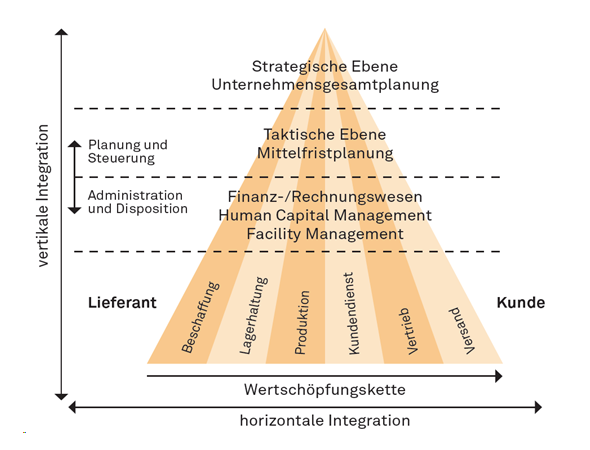
\includegraphics[width=\linewidth]{content/images/integrations-pyramide}\
    \quelle\url{http://www.referenzportal.ch/fuehrung/vom-erp-zum-integrierten-informationssystem/}
    \caption[Darstellung einer typischen Integrations-Pyramide]{Darstellung einer typischen Integrations-Pyramide\\}
    \label{fig:integrations-pyramide} 
\end{figure} 

Die Geschäftsführung der GmbH hat bereits als Software-Entwickler in anderen Unternehmen Erfahrung mit dem Umgang und den Aufbau von E-Commerce-Shops gesammelt. Zu den Erfahrungen zählen unter anderem das programmieren, testen, deployen und weiterentwickeln der Anwendung. Während dieser Prozesse sind die Programmierer zur Erkenntnis gelangt, das bei steigender Größe der Anwendung, die Aufwände für Wartung und Weiterentwicklung stark ansteigen. Dies war auch der Grund warum das Unternehmen irgendwann Insolvenz anmelden musste. Die Kosten für Wartung und einer zeitnahen Reaktion auf die Veränderungen der Nutzerbedürfnisse konnten nicht mehr getragen werden und Anbieter wie Amazon, welche deutlich schneller als das eigene Unternehmen agieren konnten, haben die Produkte des Unternehmens schließlich vom Markt gedrängt.

Aus diesem Grund möchte die Geschäftsführung der neugegründeten \gmbh\ eine Software-Architektur wählen, welches schneller anpassbar und einfacher zu warten ist. Für sie kommen daher das Microservice-Modell oder das \SOA -Modell infrage.

\section{Vorgehen und Kapitel}
\label{sec:vorgehen}
Zunächst werden die Probleme bei der Verwendung von Monolithischen Architekturmodellen, unter dem Aspekt der Softwareentwicklung und Wartung analysiert. Darauf aufbauend soll die Grundlegende Problematik herausgearbeitet werden. Anschließend werden die Grundlagen zur Verwendung von Service orientierten Architekturen und deren Vorteile, aufbauend auf die zuvor erläuterte Problematik, erklärt. In den Grundlagen werden außerdem Werkzeuge erklärt, mit deren Hilfe solche Architekturen realisiert werden können und die Wartung vereinfachen.
\\
Darauf folgend wird das Architekturmodell "'Microservice"' unter der Verwendung von den erläuterten Werkzeugen erklärt und der Begriff Continuous Delivery eingeführt. Anschließend wird, unter Verwendung des angeeigneten Wissens aus dem Kapitel "'Microservice"', auf das Architekturmodell "'Service-orientierte Architektur (SOA)"' eingegangen.
\\
Abschließend werden die gewonnen Kenntnisse zusammengetragen und Ausgewertet. Dabei sollen beide Architekturmodelle verglichen und bewertet werden. Zuletzt wird das Thema noch einmal zusammengefasst und ein Ausblick auf kommende Projekte bzw. die Bachelorarbeit gegeben.